\documentclass[10pt,a4paper]{article}
\usepackage[utf8]{inputenc}
\usepackage[spanish]{babel}
\usepackage{amsmath}
\usepackage{amsfonts}
\usepackage{amssymb}
\usepackage{graphicx}
\usepackage[left=2cm,right=2cm,top=2cm,bottom=2cm]{geometry}



\title{Reporte de artículo\\Análisis Complejo}
\author{N. Pérez Medina.}


\begin{document}
\maketitle
\begin{center}
	\textbf{Catedrático:} Haydey Alvarez Allende \\
	\\
	
\includegraphics[scale=0.05]{fing-escudo-bw.png} 
\end{center}
\newpage
\section{Introducción.}

La córnea contiene fibras de colágeno organizadas de forma muy precisa, lo que permite que la luz se propague con mínima dispersión y, en consecuencia, que podamos ver con claridad. Sin embargo, ciertas patologías corneales alteran esta estructura, provocando un aumento en la dispersión de la luz, lo cual reduce la transparencia de la córnea y afecta la calidad de la visión.

El artículo aborda este fenómeno desde un enfoque matemático y computacional. Para ello, se utilizan las ecuaciones de Maxwell, un sistema de ecuaciones diferenciales parciales que describe cómo se propaga la luz a través de medios materiales, en este caso, los tejidos de la córnea. (Especificamente una parte de la cornea llamada estorma)

Para simplificar el problema, se considera una representación de dos dimenciones de la córnea. El modelo incluye condiciones iniciales y de frontera que simulan la entrada de un pulso de luz, y se resuelve mediante métodos numéricos. En particular, se utiliza una combinación del método de Galerkin discontinuo para discretización espacial y Runge-Kutta para la evolución temporal de la solución.

\section{Contexto físico del problema}

\begin{center}
	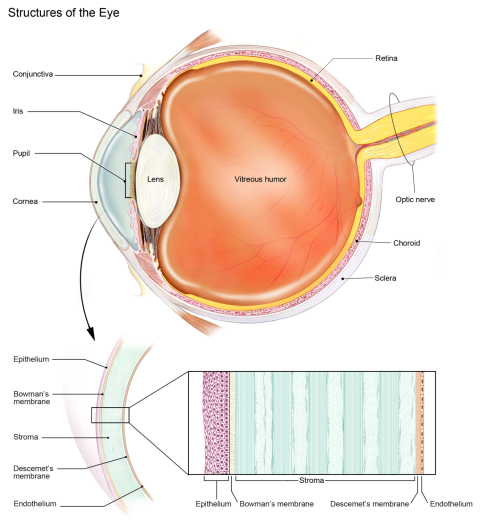
\includegraphics[scale=0.5]{partes-ojo.png} 
\end{center}

Antes de que la luz llegue a la retina para ser interpretada por nuestro sistema visual, atraviesa la córnea, una estructura transparente ubicada en la parte frontal del ojo. La córnea está compuesta por varias capas, entre las cuales el aretículo se enfoca en el estroma.

El estroma está formado por fibras de colágeno organizadas de manera estructurada y regular. Este ordenamiento específico permite que, aunque la luz se disperse al atravesar este medio, dicha dispersión ocurra de forma controlada, lo que preserva la transparencia y garantiza una buena visión.

Sin embargo, existen patologías corneales que alteran esta organización del estroma. Cuando la estructura de las fibras se afecta, la luz se dispersa de manera distinta, reduciendo la transparencia y deteriorando la calidad de la visión.

Comprender cómo y en qué medida estas alteraciones estructurales afectan la propagación de la luz es importante para evaluar el impacto en la vista de las enfermedades corneales.

\newpage

\section{Formulación matemática del modelo}

Para estudiar cómo se comporta la luz al pasar por la córnea, el artículo utiliza las ecuaciones de Maxwell, que son un conjunto de ecuaciones diferenciales que describen cómo cambian en el tiempo y en el espacio los campos eléctricos y magnéticos. 
\[
\begin{aligned}
- \nabla \times \mathbf{E} &= \epsilon \frac{\partial \mathbf{H}}{\partial t} \\
\nabla \times \mathbf{H} &= \mu \frac{\partial \mathbf{E}}{\partial t}
\end{aligned}
\]

Como trabajar con las ecuaciones completas en tres dimensiones puede ser muy costoso computacionalmente, se simplifica el problema considerando una versión en dos dimensiones. Esta reducción se basa en suponer que la propagación ocurre principalmente en un plano. Además, se usa algo llamado modo TE (transversal eléctrico), que básicamente significa que el campo eléctrico solo tiene componentes dentro del plano que se está estudiando, y que el campo magnético apunta perpendicularmente a ese plano. El artículo expresa lo anterior como 

\[
\begin{aligned}
\mathbf{E}=(E_x,E_y)\\
\mathbf{H}=(H_z)
\end{aligned}
\]

Otro punto importante es que el modelo toma en cuenta que la córnea no responde igual en todas las direcciones. Por eso, en lugar de usar un solo valor para la permitividad eléctrica (que reoresenta las propiedades de la córnea), se usa una matriz o tensor que representa cómo varía esa propiedad según la dirección. Esto es lo que se conoce como una permitividad anisotrópica. El artículo expresa lo anterior como 

\[
\varepsilon =
\begin{pmatrix}
\varepsilon_{xx} & \varepsilon_{xy} \\
\varepsilon_{yx} & \varepsilon_{yy}
\end{pmatrix}
\]

Finalmente, para resolver el problema se definen condiciones iniciales (en este caso, sin campos presentes), y condiciones de frontera, que sirven para que la onda que se simula no se refleje artificialmente en los bordes del dominio. Estas últimas se conocen como condiciones de Silver-Müller.

\section{Métodos numéricos utilizados}

Como el sistema de ecuaciones diferenciales que se plantea en el modelo no se puede resolver de forma exacta, se utilizan métodos numéricos para aproximar su solución. En el artículo se aplican dos técnicas que nunca había visto, pero se relacionan con algunas cosas que sí hemos visto en la carrera.

Primero, para resolver el problema en el espacio, se usa el método de Galerkin discontinuo. Según investigué, este método es una variante del método de elementos finitos, pero con la diferencia de que permite que la solución sea discontinua entre los elementos de la malla. 

Para resolver el problema en el tiempo, se utiliza un método de Runge-Kutta de bajo almacenamiento, también llamado LSERK por sus siglas en inglés (Low-Storage Explicit Runge-Kutta). Por lo que entendí, este es un tipo de Runge-Kutta que está optimizado para usar menos memoria en las simulaciones. Aunque es una técnica que no hemos visto, cumple la misma función básica que los Runge-Kutta que sí conocemos: aproximar soluciones paso a paso en el tiempo.

\section{Simulaciones y resultados}
\begin{center}
	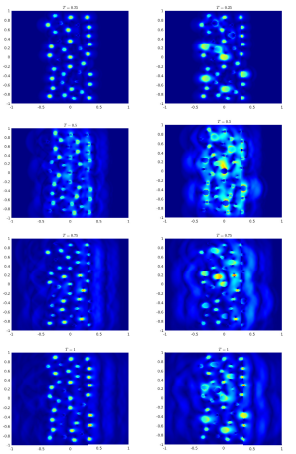
\includegraphics[scale=1]{resultados-corneas.png} 
\end{center}
En las imágenes presentadas en el artículo, se puede observar claramente la diferencia entre una córnea sana (lado izquierdo) y una córnea con alteraciones patológicas (lado derecho). En el caso de la córnea sana, la simulación muestra que, a lo largo del tiempo, la luz mantiene una propagación uniforme y con una dispersión mínima. En contraste, el lado derecho, que representa una córnea donde algunas fibras han aumentado su diámetro, se nota cómo la dispersión de la luz cambia con el tiempo.
 
En este caso, se muestra cómo una modificación aparentemente pequeña puede tener un impacto visual importante, algo que sería muy difícil de analizar sin un modelo matemático que relacione todas estas variables.
\end{document}